\chapter{Previous Work}
\section{OPEN Meter Project}
\subsection{Introduction}
The Open Public Extended Network (OPEN) meter project is a EU project with an aim to specify a comprehensive set of open and public standards for Automated Metering Infrastructure (AMI), supporting electricity, gas, water and heat metering, taking into account the real conditions of the utility networks so as to allow for full implementation \cite{OPEN_mtr_link}.

Overall work of the project is divided into the following six broad tasks: 
\begin{itemize}
\item Investigation of the functional requirements and regulatory issues concerning AMI in the various European countries.
\item Review of the state-of-the art of the various technologies available, including protocols for wired, power line carrier and wireless communication media.
\item Research and development activities to ensure that the requirements of AMI will be met in a cost effective manner.
\item Development of test approaches and procedures for laboratory, compliance and field tests of the newly developed system elements.
\item Specification and proposal of a standard.
\item Dissemination of the project results to all the stakeholders, utilities, manufacturers, energy market participants and end users.
\end{itemize}

The following subsections summarize the results of the project that are relevant to this literature study.

\subsection{Regulations for Germany}

The OPEN meter project outlines the existing regulatory requirements on smart metering throughout the European countries \cite{OPEN_mtr_reg}. This section highlights the regulatory requirements of Germany.

\subsubsection{Metering Actors}

Four companies dominate the electricity market. RWE, E.ON, Vattenfall and EnBW control 90\% of the generation and almost all of the transmission market. However there are around 870 local distribution network operators. The big four represent over 50\% of the retail.

Metering services lies with electricity network operators. The operational model sees 
responsibility for metering generally lying with the distribution businesses, although some of the larger utilities may use in-house operations for installation and reading meters.

The gas market for distribution and retail is dominated by the 5 large gas trading and retail companies – E.ON-Ruhrgas, RWE, EWE, ENBW and Vattenfall.

\subsubsection{Regulatory Framework}

The regulatory authority in Germany is  the  Federal  Network  Agency  for  Electricity,  Gas, Telecommunications, Posts and Railway (BnetzA). For smaller utilities the regulation is carried out by local (state) regulators.

Both gas and electricity markets were fully opened to competition in 1998. However in both markets, there has not been a great deal of activity due mainly to the high level of vertical and horizontal integration in the energy markets, and the emergence of a number of dominant participants. Residential switching runs at about 5\% for electricity, with gas switching numbers negligible.

\subsubsection{Functional and technical requirements}
Apart from the non-existence of legal direct technical requirements for smart metering, there are two main initiatives working on stating requirements:

Open Metering is a community of manufacturers of metering and related equipment and is supported by the associations FIGAWA\footnote{Bundesvereinigung der Firmen im Gas- und Wasserfach e.V. - http://www.figawa.de/}, ZVEI\footnote{Zentralverband Elektrotechnik- und Elektronikindustrie e.V. - http://www.zvei.org/} and KNX\footnote{http://www.knx.org/}. The goal of Open Metering is the promotion of open, cross-vendor devices and interface standards and their application. Open Metering developed specifications for product compliance i.e., a defined degree of functionality and interoperability. In this context interoperable communications interfaces of consumption meters are considered. The result of this work is the Open Metering System (OMS). In particular, a cross-media standardization is sought (multi-utility).

A German initiative driven by utilities themselves is the Multi Utility Communication (MUC) initiative\footnote{http://www.m-u-c.org}. This activity started in the spring of 2007 and is being undertaken by companies in the utilities sector under the banner of a trade association - the BDEW\footnote{German Energy and Water Association - http://www.bdew.de}.

\subsection{Technological alternatives}

The OPEN meter project studies the concepts, architectures, and state-of-the art wired and wireless communications technologies, protocols and data models applicable to Automatic Meter Reading as part of an Advanced Metering Infrastructure \cite{OPEN_mtr_tech}.

Table~\ref{tab:OPEN_tech} lists the various technologies evaluated by the OPEN meter project:

\begin{table}[h!]
\begin{center}
%\resizebox{18cm}{!}{
\begin{tabular}{| p{3.5cm} | p{3.5cm} | p{3.5cm} |}
\hline
AMR Techniques & Wireless Technologies & Wire-line Technologies \\
\hline
Walk-by, Drive-by, Fixed networks \& Hybrid networks &  Wavenis, Plextex, Everblu, Bluetooth, WPAN (Zigbee, 6LoWPAN, PHY and MAC), WLAN, WiMax, GSM/GPRS/EDGE, UMTS, LTE, PMR, 2-way  radio paging, European Radio Ripple Control, Satellite Systems. & PSTN, xDSL, FTTB, FTTH, M-Bus, PLC.\\
\hline
\end{tabular}
%}
\end{center}
\caption{Different technological alternatives}
\label{tab:OPEN_tech}
\end{table}

\subsection{OPEN meter System Architecture}
The overall system architecture is designed after the selection of suitable technologies required for AMI. Figure~\ref{fig:OPEN_sys_arch} illustrates the different system components and interfaces that define teh system architecture of the OPEN meter project \cite{OPEN_mtr_arch}.
\begin{figure}[htb!]
\centering
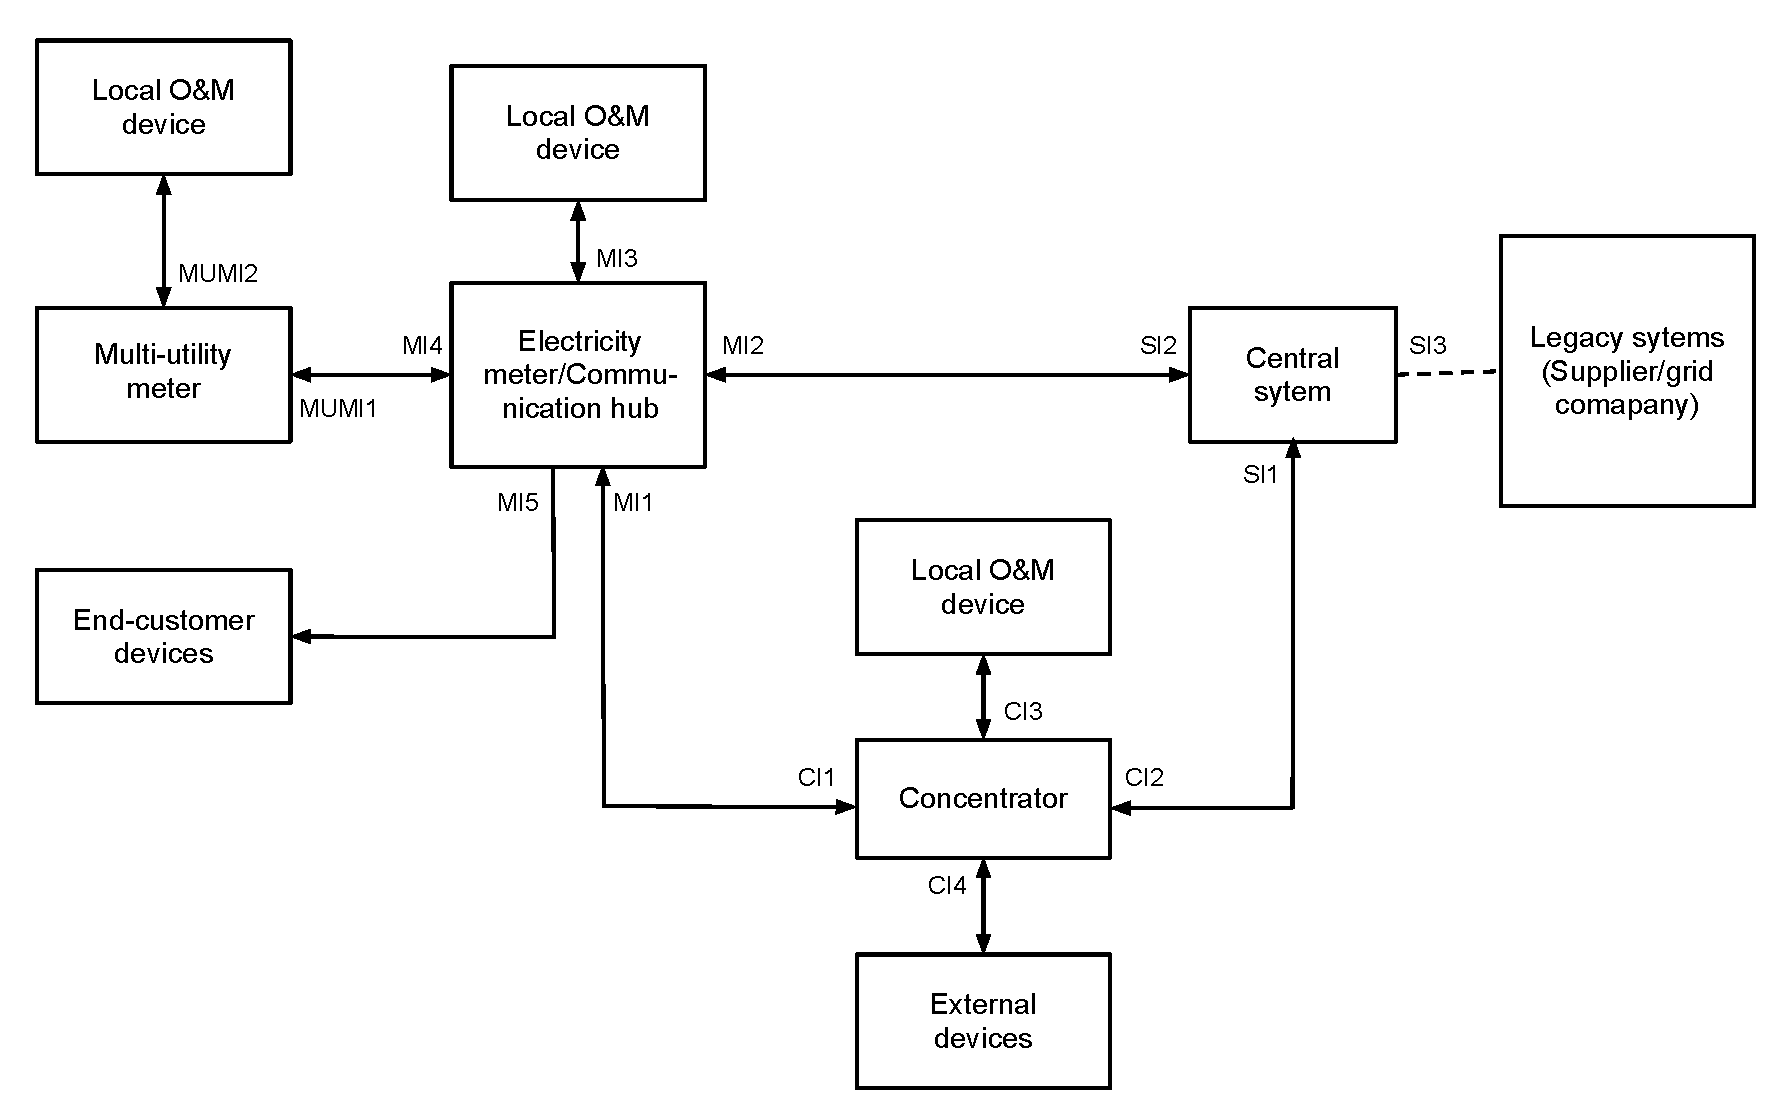
\includegraphics[width=0.8\textwidth]{images/OPEN_meter_arch}
\caption{OPEN meter system architecture \cite{OPEN_mtr_arch}.}
\label{fig:OPEN_sys_arch}
\end{figure}

\begin{table}[h!]
  \begin{center}
    \begin{tabular}{| p{3.5cm} | p{3cm} | p{4cm} |}
    \hline 
    Interface & Selected Technology Type & Lower Layer protocols \\
    \hline \hline
    MI1-CI1 & PLC & Prime, IEC 61334-5-1 \\
    \hline
    CI2-SI1 & Wireless & UMTS, GPRS \\
    \hline
    MI2-SI2 & Wireless & UMTS, GPRS \\
    \hline
    MI3, CI3 and MUMI2 & Wireless & IEE802.15.4,  IEE802.11-2007 \\
    \hline
    MUMI1-MI4 & Wireless & IEE802.15.4,  IEE802.11-2007, Wireless M-Bus \\
    \hline
    CI4 & Wireless & Zigbee, WiFi \\
    \hline
    MI5 & Wireless & Bluetooth, Zigbee \\
    \hline
    \end{tabular}
  \end{center}
  \caption{Technologies for the interfaces}
  \label{tab:OPEN_intf}
\end{table}

Electricity meter can act as a communication hub for other meters in the house and hence other meters could delegate certain power-intensive operations to the electricity meter such as cryptographic functions. The concentrator is need when the local n/w uses power line communications as a media. Local O\&M devices are used by the utilities personnel to locally configure, operate and maintain the meters and other electronic devices of the architecture. Table~\ref{tab:OPEN_intf} lists the various technologies chosen for the different interfaces in the system architecture.

Security is taken care by the DLMS/COSEM protocols. DLMS or Device Language Message Specification, is the suite of standards developed and maintained by the DLMS User Association and has been co-opted by the IEC TC13 WG14 into the IEC 62056 series of standards. COSEM or Companion Specification for Energy Metering, includes a set of specifications that defines the Transport and Application Layers of the DLMS protocol. 